%  This file is part of the ParaNut project.
% 
%  Copyright (C) 2010-2020 Alexander Bahle <alexander.bahle@hs-augsburg.de>
%						   Anna Pfuetzner <annakerstin.pfuetzner@gmail.com>
%						   Christian Meyer <Christian.Meyer@hs-augsburg.de>
%						   Gundolf Kiefer <gundolf.kiefer@hs-augsburg.de>
%      Hochschule Augsburg, University of Applied Sciences
%
% Redistribution and use in source and binary forms, with or without modification, 
% are permitted provided that the following conditions are met:
% 
% 1. Redistributions of source code must retain the above copyright notice, this 
%    list of conditions and the following disclaimer.
% 
% 2. Redistributions in binary form must reproduce the above copyright notice,
%    this list of conditions and the following disclaimer in the documentation and/or
%    other materials provided with the distribution.
%
% THIS SOFTWARE IS PROVIDED BY THE COPYRIGHT HOLDERS AND CONTRIBUTORS "AS IS" AND 
% ANY EXPRESS OR IMPLIED WARRANTIES, INCLUDING, BUT NOT LIMITED TO, THE IMPLIED 
% WARRANTIES OF MERCHANTABILITY AND FITNESS FOR A PARTICULAR PURPOSE ARE 
% DISCLAIMED. IN NO EVENT SHALL THE COPYRIGHT HOLDER OR CONTRIBUTORS BE LIABLE FOR
% ANY DIRECT, INDIRECT, INCIDENTAL, SPECIAL, EXEMPLARY, OR CONSEQUENTIAL DAMAGES 
% (INCLUDING, BUT NOT LIMITED TO, PROCUREMENT OF SUBSTITUTE GOODS OR SERVICES; 
% LOSS OF USE, DATA, OR PROFITS; OR BUSINESS INTERRUPTION) HOWEVER CAUSED AND ON 
% ANY THEORY OF LIABILITY, WHETHER IN CONTRACT, STRICT LIABILITY, OR TORT 
% (INCLUDING NEGLIGENCE OR OTHERWISE) ARISING IN ANY WAY OUT OF THE USE OF THIS 
% SOFTWARE, EVEN IF ADVISED OF THE POSSIBILITY OF SUCH DAMAGE.


%% LyX 2.2.2 created this file.  For more info, see http://www.lyx.org/.
%% Do not edit unless you really know what you are doing.
\documentclass[12pt,english,pointednumbers,liststotoc,idxtotoc]{scrreprt}
\usepackage[T1]{fontenc}
\usepackage[latin9]{inputenc}
\usepackage[a4paper]{geometry}
\geometry{verbose,tmargin=25mm,bmargin=30mm,lmargin=25mm,rmargin=25mm}
\usepackage{fancyhdr}
\pagestyle{fancy}
\setcounter{secnumdepth}{3}
\setcounter{tocdepth}{3}
\usepackage{array}
\usepackage{verbatim}
\usepackage{makeidx}
\makeindex
\usepackage{graphicx}
\usepackage{setspace}
\usepackage{xcolor}
\usepackage{multirow}
\usepackage[most]{tcolorbox}
\definecolor{consolecolor}{RGB}{220,220,220}
\newcommand{\consolebox}[1]{\par\hspace{0.25cm}\colorbox{consolecolor}
	{\texttt{#1}}\newline}
\providecommand{\gitversion}[1]{ - }
\makeatletter

%%%%%%%%%%%%%%%%%%%%%%%%%%%%%% LyX specific LaTeX commands.
%% Because html converters don't know tabularnewline
\providecommand{\tabularnewline}{\\}

%%%%%%%%%%%%%%%%%%%%%%%%%%%%%% User specified LaTeX commands.
% [From the LyX User Guide]...

\usepackage{ifpdf} % part of the hyperref bundle
\ifpdf % if pdflatex is used

% set fonts for nicer pdf view
\IfFileExists{lmodern.sty}{\usepackage{lmodern}}{}

% link all cross references and URLs in pdf output
\usepackage[colorlinks=true, bookmarks, bookmarksnumbered,
linkcolor=black, citecolor=black, urlcolor=blue, filecolor=blue,
pdfpagelayout=OneColumn, pdfnewwindow=true,
pdfstartview=XYZ, plainpages=false, pdfpagelabels,
pdfauthor={Gundolf Kiefer}, pdftex,
pdftitle={ParaNut},pdfsubject={ParaNut},
pdfkeywords={ParaNut}]{hyperref}

\else % if dvi or ps is produced

% link all cross references and URLs in dvi output
\usepackage[ps2pdf]{hyperref}

\fi % end if pdflatex is used

% the pages of the TOC are numbered roman
% and a pdf-bookmark for the TOC is added
\pagenumbering{roman}
\let\myTOC\tableofcontents
\renewcommand\tableofcontents{%
	\pdfbookmark[1]{Contents}{}
	\myTOC
	\cleardoublepage
	\pagenumbering{arabic} }

% define a short command for \textvisiblespace
\newcommand{\spce}{\textvisiblespace}

% redefine the greyed out note
%\renewenvironment{lyxgreyedout}
% {\textcolor{blue}\bgroup}{\egroup}


% [GK] ...

% Headings and footers...
\fancyhead[L]{\slshape \leftmark}
\fancyhead[C,R]{}
\fancyfoot[L]{The \paranut Processor, Gundolf Kiefer et al., \today}
\fancyfoot[C]{}
\fancyfoot[R]{\thepage}

\renewcommand{\footrulewidth}{0.6pt}
\renewcommand{\headrulewidth}{0.6pt}

\fancypagestyle{plain}{
	\fancyhead[L,C,R]{}
	\renewcommand{\headrulewidth}{0pt}
} 

%\newcolumntype{d}[1]{D{.}{.}{#1}}
% New column types to use in tabular environment for instruction formats.
% Allocate 0.18in per bit.
\newcolumntype{I}{>{\centering\arraybackslash}p{0.18in}}
% Two-bit centered column.
\newcolumntype{W}{>{\centering\arraybackslash}p{0.36in}}
% Three-bit centered column.
\newcolumntype{F}{>{\centering\arraybackslash}p{0.54in}}
% Four-bit centered column.
\newcolumntype{Y}{>{\centering\arraybackslash}p{0.72in}}
% Five-bit centered column.
\newcolumntype{R}{>{\centering\arraybackslash}p{0.9in}}
% Six-bit centered column.
\newcolumntype{S}{>{\centering\arraybackslash}p{1.08in}}
% Seven-bit centered column.
\newcolumntype{O}{>{\centering\arraybackslash}p{1.26in}}
% Eight-bit centered column.
\newcolumntype{E}{>{\centering\arraybackslash}p{1.44in}}
% Ten-bit centered column.
\newcolumntype{T}{>{\centering\arraybackslash}p{1.8in}}
% Twelve-bit centered column.
\newcolumntype{M}{>{\centering\arraybackslash}p{2.2in}}
% Sixteen-bit centered column.
\newcolumntype{K}{>{\centering\arraybackslash}p{2.88in}}
% Twenty-bit centered column.
\newcolumntype{U}{>{\centering\arraybackslash}p{3.6in}}
% Twenty-bit centered column.
\newcolumntype{L}{>{\centering\arraybackslash}p{3.6in}}
% Twenty-five-bit centered column.
\newcolumntype{J}{>{\centering\arraybackslash}p{4.5in}}

\tcbset{
    colback=gray!15,
	width=0.94\textwidth,
	colframe=gray!25,
	arc=0mm,
    }
\newenvironment{commentary}
{ 	\begin{center}
	\begin{tcolorbox}
	\small \em
		
	}
	{	
	\end{tcolorbox}
	\end{center}
}

\newcommand{\wunits}[2]{\mbox{#1\,#2}}

%\usepackage{graphicx} % part of the hyperref bundle
\newcommand{\paranut}{\mbox{\em ParaNut }}

\renewcommand{\caplabelfont}{\bf}

\makeatother

\usepackage{float}
\usepackage{babel}
\usepackage{listings}
\usepackage{xcolor}
\renewcommand{\lstlistingname}{Listing}
\definecolor{lstBackground}{RGB}{220,220,220}
\definecolor{colKeys}{rgb}{0,0,1}
\definecolor{colIdentifier}{rgb}{0,0,0}
\definecolor{colComments}{rgb}{1,0,0}
\definecolor{colString}{rgb}{0,0.5,0}
\lstset{
	float=hbp,
	basicstyle=\ttfamily\color{black}\small,
	identifierstyle=\color{colIdentifier},
	keywordstyle=\color{colKeys},
	stringstyle=\color{colString},
	commentstyle=\color{colComments},
	columns=flexible,
	tabsize=2,
	frame=single,
	extendedchars=true,
	showspaces=false,
	showstringspaces=false,
	numbers=left,
	numberstyle=\tiny,
	breaklines=true,
	backgroundcolor=\color{lstBackground},
	breakautoindent=true
}

\newcommand{\instbit}[1]{\mbox{\scriptsize #1}}
\newcommand{\instbitrange}[2]{~\instbit{#1} \hfill \instbit{#2}~}



\begin{document}

	\pagenumbering{roman}
	
	\sloppy
	
	\begin{titlepage}
		
		\begin{flushright}
			
\includegraphics[width=5cm]{figs/hsa_logo}
			\par\end{flushright}
		
		\begin{center}
			\vfill ~ \vfill
			\par\end{center}
		
		\begin{doublespace}
			\begin{center}
				\textsf{\textbf{\Huge{}The \paranut Processor}}
				\par\end{center}{\Huge \par}
			
			\begin{center}
				\textsf{\textbf{\large{}Architecture Description and Reference Manual}}
				\par\end{center}{\large \par}
		\end{doublespace}
		
		\begin{center}
			
\includegraphics[width=5cm]{figs/pn_logo}

			\textsf{\vfill}
			\par\end{center}
		
		\begin{center}
			\textsf{\LARGE{}Gundolf Kiefer, Alexander Bahle, Christian H. Meyer, Felix Wagner}
			\par\end{center}{\LARGE \par}
		
		\begin{center}
			\textsf{\large{}Hochschule Augsburg \textendash{} University of Applied
				Sciences}\\
			\par\end{center}{\large \par}
		
		\begin{center}
			\texttt{\large{}gundolf.kiefer@hs-augsburg.de}
			\par\end{center}{\large \par}

		\begin{center}
			\textsf{
				\large{}With contributions by: \\
					Michael Sch\"aferling, Anna Pf\"utzner, Patrick Zacharias
			}
			\par\end{center}{\large \par}
		
		
		\begin{center}
			\textsf{\vfill}
			\par\end{center}
		
		\begin{center}
			\textsf{\large{}Version: \gitversion}
			\par\end{center}{\LARGE \par}

		\begin{center}
			\textsf{\large{}\today \\}
			\par\end{center}{\large \par}

		\begin{center}
			\vfill ~ \vfill
			\par\end{center}

		\begin{center}
			\framebox{
				
\includegraphics[scale=0.8]{figs/cc-by-sa.png}
				~
				\parbox{12cm}{\footnotesize This work is licensed under a Creative Commons Attribution-ShareAlike 4.0 International License. To view a copy of this license, visit https://creativecommons.org/licenses/by-sa/4.0/.}
			}
			\par\end{center}

	\end{titlepage}

\begin{comment}
~

NOTE: Run 'make lyxdeps' to update all figures and the instruction
set directory!

~
\end{comment}


\chapter*{Document History}

\begin{tabular}{|c|c|p{11cm}|}
	\hline
	\textbf{Version} & \textbf{Date} & \textbf{Description}\tabularnewline
	\hline
	\hline
	0.2.0            & 2015-02-19    & Initial public release\tabularnewline
	\hline
	0.2.1            & 2015-12-16    & Add local CPU identification register, LL/SC instructions\tabularnewline
	\hline
	0.3.0            & 2018-12-01    & Change to RISC-V ISA \tabularnewline
	\hline
	0.3.1            & 2020-11-16    & Minor improvements\tabularnewline
	\hline
	0.4.0            & 2020-02-08    & Add User and Supervisor modes  \tabularnewline
	\hline
	0.4.1            & 2020-11-16    & Minor improvements\tabularnewline
	\hline
	0.4.2            & 2021-05-26    & Minor improvements\tabularnewline
	\hline
	1.0.0            & 2021-11-22    & Major rework of the manual, avoiding duplication of general RISC-V information;\par Switch to Git-based versioning\tabularnewline
	\hline
	                 &               & \tabularnewline
	\hline
\end{tabular}

\tableofcontents{}

\chapter{Introduction}

The goal of the \paranut project is to develop an open, scalable
and practically applicable multi-core processor architecture for embedded
systems. Scalability is given by supporting parallelism at thread
and data level based on multiple processing cores while keeping the
design of the individual core itself as simple as possible.

\paranut introduces a unique concept for SIMD (single instruction,
multiple data) vectorization. Whereas SIMD extensions for workstation
processors or embedded systems frequently contain specialized instructions
leading to an inherently bad compiler support, SIMD code for the \paranut
can be programmed in a high-level language according to a paradigm
very similar to thread programming.

The instruction set is kept compatible to the RISC-V specification.
Hence, the RISC-V GCC tool chain and libraries/operation systems
(newlib, Linux in the future with some necessary extensions) can be used with the
\paranut.

To date, the \paranut project is still work in progress, and new
contributors from industry and academia are welcome. An informal project
overview including the implementation status and very promising benchmark
results can be found in \cite{Kief15}.

\chapter{The \paranut Architecture}

\section{Instruction Set Architecture}

The \paranut instruction set architecture is compatible with the
RISC-V specification. The RISC-V architecture is an open source
load and store RISC architecture designed with the purpose
to support a wide spectrum of different chips from small microcontrollers to server CPUs. \cite{userspec}.
Scalability is achieved by defining a minimalistic basic instruction
set (RV32I) together with optional extensions including a floating-point
unit (FPU) or a memory management unit (MMU). Furthermore, the basic
architecture offers configuration options such as different register
file sizes or optional arithmetic instructions.

\paranut processors implement all mandatory instructions according
to the RV32I specification. Features unique to \paranut require
some additional \paranut-specific instructions. These will be encapsulated
in a small support library, so that they are still usable without
compiler modifications. For software development, the GCC tool chain
from the RISC-V project can be used without any modifications. A
cycle-accurate SystemC model can be used as an instructions set simulator.
To date, an operating environment based on the \textquotedbl{}newlib\textquotedbl{}
C library allows to compile and run software both in the simulator
and on real hardware.

\section{Structural Organisation}

The general structure of \paranut is depicted in Figure \ref{fig:paranut_architecture}.
The core contains one \emph{Central Processing Unit (CePU)} and a
number of \emph{Co-Processing Units (CoPU)}. The CePU is a full-featured
CPU, whereas the CoPUs are CPUs with a more or less reduced functionality
and complexity. Depending on the mode of execution (see below), the
CoPUs may either be inactive (sequential code), execute a part of
a vector operation, or execute a thread. In the sequel, the term CPU
refers to any of a CePU or a CoPU.

All the CPUs are connected to a central \emph{Memory Unit (MemU)}.
The MemU contains the cache(s) and means to support synchronisation
primitives. It provides a single bus interface to the main system
bus, and independent read and write ports for each CPU. It is optimized
to support parallel accesses by different CPUs. In particular, multiple
read accesses to the same address can be served in parallel and run
no slower than a single access, and accesses to neighboring addresses
can mostly be served in parallel. These two properties are particularly
important for the SIMD-like mode.

\begin{figure}
	\noindent \begin{centering}
		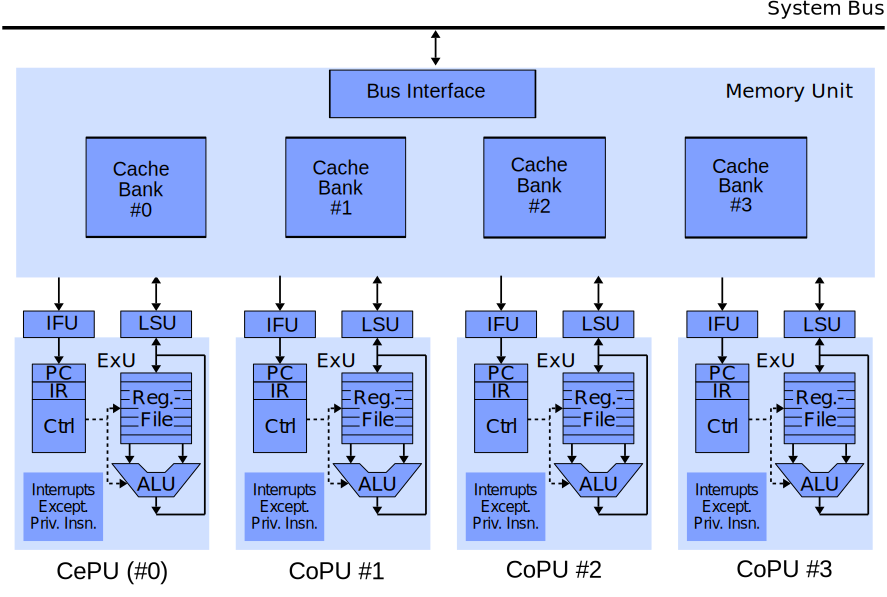
\includegraphics[width=15cm]{figs/paranut-0-4_cores}
		\par\end{centering}
	\caption{A \paranut instance with 4 cores\label{fig:paranut_architecture}}
\end{figure}

Each CPU contains an ALU, a register file and some control logic which
together form the \emph{Execution Unit (ExU)}. The \emph{Instruction
	Fetch Unit (IFU)} is responsible for fetching instructions from the
memory subsystem and contains a small buffer for prefetching instructions.
The \emph{Load-Store Unit (LSU)} is responsible for performing the
data memory accesses of load and store operations. It contains a small
store buffer and implements write combining and store forwarding mechanisms
as well as mechanisms to support atomic operations.

The Execution Unit is designed and optimized for a best-case throughput
of one instruction in two clock cycles (CPI$\approx$2,
CPI = \textquotedbl{}clocks per instruction\textquotedbl{}). This
is slower than modern pipeline designs targeting a best-case CPI value
of 1. However, it allows to better optimize the execution unit for
area, since no pipeline registers or extra components for the detection
and resolution of pipeline conflicts are required. Furthermore, in
a multi-core system, the performance is likely to be limited by bus
and memory contention effects anyway, so that an \emph{average} CPI
value of 1 is expected to be hardly achievable in practice. In the
\paranut design, several measures help to maintain an average-case
throughput very close to the best-case value of CPI$\approx$2,
even for multi-core implementations.

The design of the memory interface and cache organization is very
critical for the scalability of many-core systems. In a \paranut
system, the Memory Unit (MemU) contains the cache, the system bus
interface, and a multitude of read and write ports for the processor
cores. Each core is connected to the MemU by two independent read
ports for instructions and data and one write port for data. The cache
memory logically operates as a shared cache for all cores and is organized
in independent banks with switchable paths from each bank to each
read and write port. Tag data is replicated to allow arbitrary concurrent
lookups. Parallel cache data accesses by different ports can be performed
concurrently if their addresses a) map to different banks or b) map
to the same memory word in the same bank. Furthermore, by using dual-ported
Block-RAM cells, each bank can be equipped with two ports, so that
up to two conflicting accesses (i.e. same bank, different
addresses) are possible in parallel. Hence, even for many cores, the
likelihood of contention can be arbitrarily reduced by increasing
the number of banks, which is configurable at synthesis time.

The cache can be configured to be 1/2/4-way set associative with configurable
replacement strategies (e.g. pseudo-random or least-recently used).
The Memory Unit implements mechanisms for uncached memory accesses
(e.g. for I/O ports) and support for atomic operations. All transactions
to and from the system bus are handled by a bus interface unit, which
presently supports the Wishbone bus standard, but can easily be replaced
to support other busses such as AXI.

\section{Execution Modes and Capabilities}

A CPU in the \paranut architecture can run in 4 different modes:
\begin{labeling}{00.00.0000}
	\item [{Mode~0~(Halted):}] The CPU is inactive.
	\item [{Mode~1~(Linked):}] The CPU does not fetch instructions, but executes
	the instruction stream fetched by the CPU.
	\item [{Mode~2~(Unlinked):}] The CPU fetches and executes its own instructions.
	Exceptions trigger an exception of the controlling CePU and put this
	CPU into Mode 0. The CePU can later put this CPU into Mode 2 again,
	and the code execution continues as if the exception has been handled
	by this CPU.
	\item [{Mode~3~(Autonomous):}] The CPU executes its own instructions.
	Exceptions and interrupts can be handled by this CPU.
\end{labeling}
Typically, the CePU always runs in Mode~3. The mode of the CoPUs
is controlled by the CePU. Depending on the application, the CoPUs
can be customized that they only support a subset of the 4 modes.
For example, if only SIMD vectorization and no multi-threading is
required, all the logic required for modes 2 and 3 can be stripped
off. Now, the CoPU does not require much more area than a vector slice
of a normal SIMD unit would. In general, a CoPU is customized for
a \emph{capability level} of $m$, meaning that all modes $\leq m$
are supported.
\begin{itemize}
	\item A Capability-1-CoPU only contains very little logic besides the ALU
	      and the register file. Hence, a \paranut with only Capability-1-CoPUs
	      does not require much more area than a normal SIMD processor.
	\item A Capability-2-CoPU additionally contains an instruction fetch unit
	      and eventually one more read port to the Memory Unit (MemU) for it.
	\item A Capability-3-CoPU is basically a full-featured CePU. It contains
	      logic to handle interrupts and exceptions and has its own set of special
	      registers. This is not needed for multi-threading, but for multi-processing,
	      where each CoPU is managed by the operating system as an individual
	      CPU.
\end{itemize}
A CPU with Capability $\geq$2 in Mode~0 will reset its IFU. Upon changing to Mode~2 or higher the CPU starts executing at the reset vector address. This enables control of Mode~2 CoPUs through software. Figure \ref{fig:paranut-all_modes} illustrates the active/required
hardware for the 4 modes. The following sections briefly illustrate
how SIMD vectorization or multi-threading can be performed. Further
informal explanations and examples can be found in \cite{Kief15}.

\begin{figure}
	\noindent \begin{centering}
		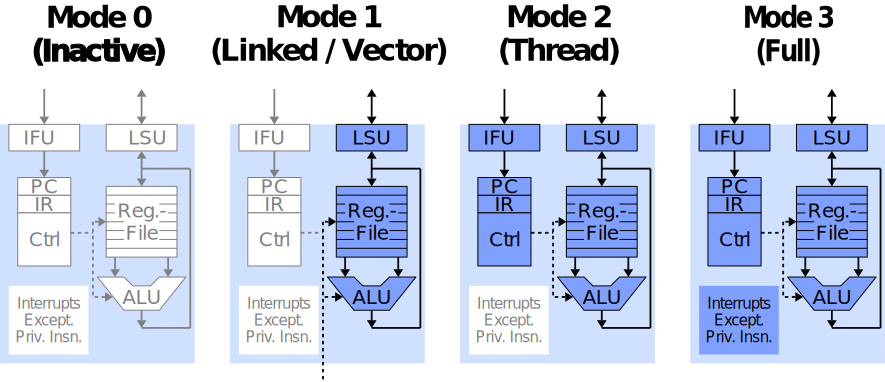
\includegraphics[width=15cm]{figs/paranut-2-all_modes}

		\par\end{centering}
	\caption{\paranut modes and required logic\label{fig:paranut-all_modes}}
\end{figure}


\section{SIMD Vectorization}

In Mode~1, the CoPU performs exactly the same instructions as the
CePU. This is the SIMD mode. All registers of the CePU can be regarded
as a slice of a big vector register. Since all CPUs perform the same
operation at a time, the memory bandwidth required for instruction
fetching is reduced considerably and equivalent to the bandwith of
a single-core processor.

From a software perspective, the code on a CoPU executes almost normally,
just like multi-threaded code. There is only a single, well-defined
exception: Conditional branches and jump instructions with variable
target addresses are executed based on target address determined by
the CePU. In the C language, such critical instructions can be generated
out of ``if'' statements, ``case'' statements and loop constructs.
As long as the conditions always evaluate equally on all CPUs, SIMD
code can be easily written using a standard compiler and a thread-like
programming model. Figure \ref{fig:Vectorized-loop} shows an example
of a vectorized loop. The macros 'pn\_begin\_linked' and 'pn\_end\_linked'
open and close a parallel code section, respectively. Since the body
of the ``for'' loop does not contain any conditional branches and
the loop end condition ``n < 100'' always evaluates equally on all
CPUs, this code is executable on an SIMD-based processor variant.

\begin{figure}
	\textbf{\tiny{}}
	\begin{lstlisting}[basicstyle={\small},language=C]
		int a[100], b[100], s[100];
		
		void add_arrays_sequential () {
			for (n = 0; n < 100; n += 1)
				s[n] = a[n] + b[n];
		}
		
		void add_arrays_parallel () {
			int n, cpu_no;
			
			// Activate 3 (=4-1) CoPUs in the "Linked" state and
			pn_begin_linked (4);       
			
			//   get the number of this CPU...
			cpu_no = pn_get_cpu_no();
			
			// performs 4 additions in parallel
			for (n = 0; n < 100; n += 4)
				s[n + cpu_no] = a[n + cpu_no] + b[n + cpu_no];    
			
			// End linked mode, deactivate the CoPUs...
			pn_end_linked ();
		}   
		\end{lstlisting}
	{\tiny \par}

	\caption{Example of a vectorized loop\label{fig:Vectorized-loop}}
\end{figure}


\section{Multi-Threading}

To perform simultaneous multi-threading, the CoPUs are put
into Mode~2. In this mode, all exceptions and interrupts are handled
by the CePU. This is somewhat a limitation compared to Mode 3, in
which the CPUs operate more autonomously. However, Mode 2 is sufficient
for all typical applications, in which multi-threading is used as
an acceleration measure.

%% [[ TBD: reference to pthreads, OpenMP, ... ]]

\chapter{Instruction Set Reference\label{cha:is_ref}}
This chapter contains the instruction set reference for the \paranut achitecture.

\section{Privilege Levels}

The \paranut supports several combinations of privilege levels as specified
in the RISC-V manual \cite{privspec}, which can be set in the global configuration
setting \texttt{CFG\_PRIV\_LEVELS}. The currently supported combinations are listed
in Table~\ref{privcombs} and can be configured by setting the desired number of levels.

\begin{table*}[h!]
	\begin{center}
		\begin{tabular}{|c|l|l|}
			\hline
			Number of levels & Supported Modes & Intended Usage                              \\ \hline
			1                & M               & Simple embedded systems                     \\
			2                & M, U            & Secure embedded systems                     \\
			3                & M, S, U         & Systems running Unix-like operating systems \\
			
			\hline
		\end{tabular}
	\end{center}
	\caption{Supported combinations of privilege modes. \cite{privspec}}
	\label{privcombs}
\end{table*}

Note that the N-Extension, enabling User-mode exception and interrupt handling
is currently not supported. Furthermore, no Memory Management Unit MMU is implemented
at this time, thus no virtual address translation is possible in any mode.

\clearpage

\section{Instructions\label{sec:is_ref-instructions}}

The \paranut implements the RV32I base instruction set. It may be configured to additionally include the {\tt M} and {\tt A} extensions.
For a full list of the corresponding instructions please refer to the RISC-V Instruction Set Manual Volume I \cite{userspec}.
This chapter contains additional implementation specific information on some instructions.

\subsection{Conditional Branches}

Currently no branch prediction is featured, 
branches as well as jumps stall the instruction fetch until the condition and/or address is evaluated.

\subsection{Load and Store Instructions}

A \paranut raises the appropriate address misaligned exception on misaligned loads and stores. 
The trap is taken according to specification and the failing address is saved in \emph{mtval} 
for further handling. Misaligned stores do not cause any changes in memory. 
Misaligned loads do not change the value of \emph{rd}.


\subsection{Memory Ordering Instructions}
\label{sec:fence}

The \paranut processor operates inorder and the write buffer of the Load Store Units is emptied 
inorder so the FENCE instruction is currently implemented as a LSU flush and the IFU buffer is also cleared.


For synchronization between a \paranut processor and other hardware in the system the special cache 
control instructions described in Section \ref{sec:csr_instructions} can be used.

\subsection{Control and Status Register Instructions} \label{sec:csr_instructions}
	
SYSTEM instructions are used to access system functionality that might
require privileged access and are encoded using the I-type instruction
format.  These can be divided into two main classes: those that
atomically read-modify-write control and status registers (CSRs), and
all other potentially privileged instructions.

\subsection{Trap-Return Instructions}
\label{retinsn}

Information about these instructions can be found in the RISC-V Privileged Architecture Instruction Set Manual \cite{privspec}
\begin{commentary}
	\paranut does not implement the N-Extension, meaning URET is not supported. SRET is only available
	if S-mode is enabled.
\end{commentary}

\clearpage
\subsection{\paranut Instructions\label{sec:is_ref-paranut_instructions}}
The \paranut architecture uses the \emph{custom-0} (0x0B) major opcode for its custom instructions as suggested in the RISC-V ISA manual \cite{userspec}.\\
\vspace{-0.2in}
\begin{center}
	\begin{tabular}{M@{}R@{}F@{}R@{}S}
		\\
		\instbitrange{31}{20}         &
		\instbitrange{19}{15}         &
		\instbitrange{14}{12}         &
		\instbitrange{11}{7}          &
		\instbitrange{6}{0}                                           \\
		\hline
		\multicolumn{1}{|c|}{funct12} &
		\multicolumn{1}{c|}{rs1}      &
		\multicolumn{1}{c|}{funct3}   &
		\multicolumn{1}{c|}{rd}       &
		\multicolumn{1}{c|}{opcode}                                   \\
		\hline
		12                            & 5    & 3       & 5 & 7        \\
		0                             & 0    & HALT    & 0 & CUSTOM-0 \\
		offset[11:0]                  & base & CINV    & 0 & CUSTOM-0 \\
		offset[11:0]                  & base & CWB     & 0 & CUSTOM-0 \\
		offset[11:0]                  & base & CFLUSH  & 0 & CUSTOM-0 \\
		0                             & 0    & CINVA   & 0 & CUSTOM-0 \\
		0                             & 0    & CWBA    & 0 & CUSTOM-0 \\
		0                             & 0    & CFLUSHA & 0 & CUSTOM-0 \\
	\end{tabular}
\end{center}

The HALT instruction halts the current CPU by switching to Mode~0. If executed on the CePU it also halts \underline{all} other CPUs in the system. Note that halting a mode 2 capable CPU will cause the reset of its program counter to the reset address.\\

The CINV, CWB and CFLUSH instructions control the MemU cache. All of these operate on the effective address obtained by adding register \emph{rs1} to the sign extended 12-bit offset. CINV just invalidates the cache line containing the effective address, while CWB triggers a write back of the cache line to main memory. CFLUSH is the combination of CWB and CINV. Similarly the CINVA, CWBA and CFLUSHA serve the same function but execute it on the whole cache.

\begin{commentary}
	The CINV(A), CWB(A) and CFLUSH(A) instructions are also buffered in the LSU write buffer and are non blocking. They can take an arbitrary amount of time to complete. If you need the instruction to complete before continuing the execution follow it with a ''fence'' instruction to ensure the cache operation is fully executed.
\end{commentary}

\pagebreak

\section{Control and Status Registers (CSR)\label{sec:is_ref-special_purpose_registers}}

	This section describes the Control and Status Registers (CSRs), which are either
	standard machine or supervisor CSRs, or specific to the \paranut architecture.
	The addresses used are defined in the RISC-V Privileged Architecture Instruction
	Set Manual \cite{privspec}. All registers are 32 bits wide. Registers mentioned in Tables \ref{tab:machine-CSRs}, \ref{tab:supervisor-CSRs}, and \ref{tab:paranut-CSRs} 
	are readable only by the \emph{CePU}.
	
	The descriptions, tables and figures in Sections \ref{field}, \ref{machine} and \ref{supervisor} are derived from the RISC-V privileged ISA \cite{privspec}. Clarifications or deviations from the specification are added as comments. 
	
	
	\subsection{Terminology and Conventions for CSR Field Specifications} 
	\label{field}
	Tables \ref{tab:csr_abbriviations} and \ref{tab:privilege_abbriviations} list abbreviations frequently used in this chapter. A more detailed description of 
	the abbreviations may be found in Chapter 2.3 of the RISC-V Privileged Architecture Instruction Set Manual \cite{privspec}.
	Tables~\ref{tab:machine-CSRs}, \ref{tab:supervisor-CSRs}, and \ref{tab:paranut-CSRs} contain information about the available
	CSRs and their access restrictions.\\
\begin{table}[htb!]
	\begin{center}
		\begin{tabular}{|l|l|}
			\hline
			Abbreviation & Description                        \\
			\hline
			WIRI       & Reserved Writes Ignored, Reads Ignore Values    \\
			WPRI       & Reserved Writes Preserve Values, Reads Ignore Values             \\
			WLRL       & Write/Read Only Legal Values       \\
			WARL       & Write Any Values, Reads Legal Values                \\
			\hline
		\end{tabular}
		\caption{Write mode abbreviations}
		\label{tab:csr_abbriviations}
	\end{center}
\end{table}

\begin{table}[htb!]
	\begin{center}
		\begin{tabular}{|l|l|}
			\hline
			Privilege & Description                        \\
			\hline
			MRW       & Machine Mode Readable/Writeable    \\
			MRO       & Machine Mode Read-Only             \\
			URW       & User Mode Readable/Writeable       \\
			URO       & User Mode Read-Only                \\
			SRW       & Supervisor Mode Readable/Writeable \\
			SRO       & Supervisor Mode Read-Only          \\
			\hline
		\end{tabular}
		\caption{Privilege abbriviations}
		\label{tab:privilege_abbriviations}
	\end{center}
\end{table}


\subsection{Machine-Level Control and Status Registers}
\label{machine}

Table~\ref{tab:machine-CSRs} lists all Control and Status Registers (CSR) implemented by the \paranut
architecture. Unless mentioned otherwise, they are implemented according to the
RISC-V specification \cite{privspec}. The following subsections describe the implementation-specific
details as they are implemented on a \paranut. Note, that all registers listed in this section are solely available on the CePU. 
Trying to access them from a CoPU raises an Illegal Instruction exception.

\begin{table}[htb!]
	\begin{center}
		\resizebox{\textwidth}{!}{%
			\begin{tabular}{|l|l|l|l|}
				\hline
				Number    & Privilege & Name                        & Description                                       \\
				\hline
				\multicolumn{4}{|c|}{Machine Information Registers}                                                     \\
				\hline
				\tt 0xF11 & MRO       & \tt mvendorid               & Vendor ID.                                        \\
				\tt 0xF12 & MRO       & \tt marchid                 & Architecture ID.                                  \\
				\tt 0xF13 & MRO       & \tt mimpid                  & Implementation ID.                                \\
				\tt 0xF14 & MRO       & \tt mhartid                 & Hardware thread ID.                               \\
				\hline
				\multicolumn{4}{|c|}{Machine Trap Setup}                                                                \\
				\hline
				\tt 0x300 & MRW       & \tt mstatus                 & Machine status register.                          \\
				\tt 0x301 & MRO       & \tt misa                    & ISA and extensions                                \\
				\tt 0x302 & MRW       & \tt medeleg                 & Machine exception delegation register.            \\
				\tt 0x303 & MRW       & \tt mideleg                 & Machine interrupt delegation register.            \\
				\tt 0x304 & MRW       & \tt mie                     & Machine interrupt-enable register.                \\
				\tt 0x305 & MRW       & \tt mtvec                   & Machine trap-handler base address.                \\
				\hline
				\multicolumn{4}{|c|}{Machine Trap Handling}                                                             \\
				\hline
				\tt 0x340 & MRW       & \tt mscratch                & Scratch register for machine trap handlers.       \\
				\tt 0x341 & MRW       & \tt mepc                    & Machine exception program counter.                \\
				\tt 0x342 & MRW       & \tt mcause                  & Machine trap cause.                               \\
				\tt 0x343 & MRW       & \tt mtval                   & Machine bad address or instruction.               \\
				\tt 0x344 & MRW       & \tt mip                     & Machine interrupt pending.                        \\
				\hline
				\multicolumn{4}{|c|}{Machine Counter/Timers}                                                            \\
				\hline
				\tt 0xB00 & MRW       & \tt mcycle                  & Machine cycle counter.                            \\
				\tt 0xB02 & MRW       & \tt minstret                & Machine instructions-retired counter.             \\
				\tt 0xB03 & MRW       & \tt mhpmcounter3            & Machine performance-monitoring counter.           \\
				\tt 0xB04 & MRW       & \tt mhpmcounter4            & Machine performance-monitoring counter.           \\
				          &           & \multicolumn{1}{c|}{\vdots} & \                                                 \\
				\tt 0xB1F & MRW       & \tt mhpmcounter31           & Machine performance-monitoring counter.           \\
				\tt 0xB80 & MRW       & \tt mcycleh                 & Upper 32 bits of {\tt mcycle}, RV32I only.        \\
				\tt 0xB82 & MRW       & \tt minstreth               & Upper 32 bits of {\tt minstret}, RV32I only.      \\
				\tt 0xB83 & MRW       & \tt mhpmcounter3h           & Upper 32 bits of {\tt mhpmcounter3}, RV32I only.  \\
				\tt 0xB84 & MRW       & \tt mhpmcounter4h           & Upper 32 bits of {\tt mhpmcounter4}, RV32I only.  \\
				          &           & \multicolumn{1}{c|}{\vdots} & \                                                 \\
				\tt 0xB9F & MRW       & \tt mhpmcounter31h          & Upper 32 bits of {\tt mhpmcounter31}, RV32I only. \\
				\hline
				\multicolumn{4}{|c|}{Machine Counter Setup}                                                             \\
				\hline
				\tt 0x323 & MRW       & \tt mhpmevent3              & Machine performance-monitoring event selector.    \\
				\tt 0x324 & MRW       & \tt mhpmevent4              & Machine performance-monitoring event selector.    \\
				          &           & \multicolumn{1}{c|}{\vdots} & \                                                 \\
				\tt 0x33F & MRW       & \tt mhpmevent31             & Machine performance-monitoring event selector.    \\
				\hline
				\multicolumn{4}{|c|}{Machine Timer Registers}                                                           \\
				\hline
				\tt 0xF01 & MRW       & \tt mtime                   & Machine timer register.                           \\
				\tt 0xF02 & MRW       & \tt mtimeh                  & Upper 32 bits of {\tt mtime}                      \\
				\tt 0xF03 & MRW       & \tt mtimecmp                & Machine timer compare register.                   \\
				\tt 0xF04 & MRW       & \tt mtimecmph               & Upper 32 bits of {\tt mtimecmp}                   \\
				\hline
			\end{tabular}
		}
	\end{center}
	\caption{Currently defined standard RISC-V CSRs}
	\label{tab:machine-CSRs}
\end{table}

\clearpage

\subsubsection{Machine Vendor ID Register ({\tt mvendorid})}

Returns a fixed value of 0 indicating a non-commercial implementation as defined in \cite{privspec}.

\begin{figure*}[h!]
	{\footnotesize
		\begin{center}
			\begin{tabular}{J}
				\instbitrange{MXLEN-1}{0}       \\
				\hline
				\multicolumn{1}{|c|}{0 (Fixed)} \\
				\hline
				MXLEN                           \\
			\end{tabular}
		\end{center}
	}
	\vspace{-0.1in}
	\caption{Vendor ID register ({\tt mvendorid}).}
	\label{mvendorreg}
\end{figure*}

\subsubsection{Machine Architecture ID Register ({\tt marchid})}

Returns a fixed value of 0, since the Architecture ID is not yet requested from the RISC-V Foundation.

\begin{figure*}[h!]
	{\footnotesize
		\begin{center}
			\begin{tabular}{J}
				\instbitrange{MXLEN-1}{0}       \\
				\hline
				\multicolumn{1}{|c|}{0 (Fixed)} \\
				\hline
				MXLEN                           \\
			\end{tabular}
		\end{center}
	}
	\vspace{-0.1in}
	\caption{Machine Architecture ID register ({\tt marchid}).}
	\label{marchreg}
\end{figure*}

\subsubsection{Machine Implementation ID Register ({\tt mimpid})}

This register provides detailed Information about the ParaNut hardware revision as
shown in Figure \ref{mimpidreg}. The ParaNut versioning scheme follows the very common Major, Minor, Revision scheme. Additionally bit 0 represents a dirty
flag, indicating if the hardware has been modified.

\begin{figure*}[h!]
	{\footnotesize
		\begin{center}
			\begin{tabular}{ccEc}
				\instbitrange{31}{24}              		       &
				\instbitrange{23}{16}                 		   &
				\instbitrange{15}{1}                		   &			
				\instbit{0}                                    \\
				\hline
				\multicolumn{1}{|c|}{Major} &
				\multicolumn{1}{c|}{Minor}             &
				\multicolumn{1}{c|}{Revision}             &
				\multicolumn{1}{c|}{Dirty}          \\
				\hline
				8 & 8 & 15 & 1 \\
			\end{tabular}
		\end{center}
	}
	\vspace{-0.1in}
	\caption{Machine Implementation ID register ({\tt mimpid}).}
	\label{mimpidreg}
\end{figure*}


\subsubsection{Hart ID Register ({\tt mhartid})\label{subsec:mhartid}}

The {\tt mhartid} CSR is an MXLEN-bit read-only register containing the integer ID of
the hardware thread running the code. The RISC-V specification defines a hart as a
single hardware thread. In the current ParaNut implementation, multiple hardware threads on a single core are not supported.
Therefore, the Hart ID Register is equivalent to {\tt pncoreid}. {\tt mhartid} can only be accessed by
the CePU, which means it always returns zero.

\begin{figure*}[h!]
	{\footnotesize
		\begin{center}
			\begin{tabular}{J}
				\instbitrange{MXLEN-1}{0}     \\
				\hline
				\multicolumn{1}{|c|}{Hart ID} \\
				\hline
				MXLEN                         \\
			\end{tabular}
		\end{center}
	}
	\vspace{-0.1in}
	\caption{Hart ID register ({\tt mhartid}).}
	\label{mhartidreg}
\end{figure*}

\subsubsection{Machine Status Register ({\tt mstatus})}
\label{mstatus}

Implements the flags listed in Figure~\ref{mstatusreg-rv32}, which represent only a subset of {\tt mstatus} in \cite{privspec}.
\textit{WPRI} indicates that the bits are not yet implemented and
should be preserved on writes for forward compatibility reasons, as indicated in Table~\ref{tab:csr_abbriviations}


\begin{figure*}[h!]
	{\footnotesize
		\begin{center}
			\begin{tabular}{Ecccccccccc}
				\instbitrange{MXLEN-1}{9}           &
				\instbit{8}                         &
				\instbit{7}                         &
				\instbit{6}                         &
				\instbit{5}                         &
				\instbit{4}                         &
				\instbit{3}                         &
				\instbit{2}                         &
				\instbit{1}                         &
				\instbit{0}                                                             \\
				\hline
				\multicolumn{1}{|c|}{\textit{WPRI}} &
				\multicolumn{1}{c|}{SPP}            &
				\multicolumn{1}{c|}{MPIE}           &
				\multicolumn{1}{|c|}{\textit{WPRI}} &
				\multicolumn{1}{c|}{SPIE}           &
				\multicolumn{1}{|c|}{\textit{WPRI}} &
				\multicolumn{1}{c|}{MIE}            &
				\multicolumn{1}{|c|}{\textit{WPRI}} &
				\multicolumn{1}{c|}{SIE}            &
				\multicolumn{1}{|c|}{\textit{WPRI}}                                     \\
				\hline
				23                                  & 1 & 1 & 1 & 1 & 1 & 1 & 1 & 1 & 1 \\
			\end{tabular}
		\end{center}
	}
	\vspace{-0.1in}
	\caption{Machine-mode status register ({\tt mstatus}) for RV32.}
	\label{mstatusreg-rv32}
\end{figure*}

\subsubsection{Machine ISA Register ({\tt misa})}

The {\tt misa} CSR is a \textit{WARL} \textit{read-only} register
reporting the ISA supported by the hart. As the \paranut is highly configurable,
the Extensions filed may or may not report some extensions. Table~\ref{misaletters}
shows the possibilities of configuration. MXL is fixed to 1 to indicate 32-bit support.

\begin{figure*}[h!]
	{\footnotesize
		\begin{center}
			\begin{tabular}{c@{}c@{}L}
				\instbitrange{MXLEN-1}{MXLEN-2}                &
				\instbitrange{MXLEN-3}{26}                     &
				\instbitrange{25}{0}                                           \\
				\hline
				\multicolumn{1}{|c|}{MXL[1:0] (\textit{WARL})} &
				\multicolumn{1}{c|}{\textit{WIRI}}             &
				\multicolumn{1}{c|}{Extensions[25:0] (\textit{WARL})}          \\
				\hline
				2                                              & MXLEN-28 & 26 \\
			\end{tabular}
		\end{center}
	}
	\vspace{-0.1in}
	\caption{Machine ISA register ({\tt misa}).}
	\label{misareg}
\end{figure*}

\begin{table*}[h!]
	\begin{center}
		\begin{tabular}{|r|r|c|l|}
			\hline
			Bit & Character & Fixed/Configuration & Description                                                               \\
			\hline
			0   & A  & {\tt CFG\_EXU\_A\_EXTENSION$=$1} & Atomic extension                                                 \\
			8   & I  & Fixed to {\tt 1}      & RV32I/64I/128I base ISA                                                   \\
			12  & M  & {\tt CFG\_EXU\_M\_EXTENSION$=$1} & Integer Multiply/Divide extension                                         \\
			18  & S  & {\tt CFG\_PRIV\_LEVELS$=$3}  & Supervisor mode implemented                                               \\
			20  & U  & {\tt CFG\_PRIV\_LEVELS$\ge$2}       & User mode implemented                                                     \\
			23  & X  & Fixed to {\tt 1}      & ParaNut extensions present                                           \\
			\hline
		\end{tabular}
	\end{center}
	\caption{Encoding of Extensions field in {\tt misa}.}
	\label{misaletters}
\end{table*}

\subsubsection{Machine Interrupt Registers ({\tt mip} and {\tt mie})}

	These registers are read-write registers, but currently without any functionality. In later
	revisions they might be reworked.


	\subsubsection{Machine Trap Vector Base Address Register ({\tt mtvec})}

	Currently, the lowest two bits are fixed to zero, which indicates that all traps set the program counter to BASE+4.
	
	\begin{figure*}[h!]
		{\footnotesize
			\begin{center}
				\begin{tabular}{J@{}R}
					\instbitrange{MXLEN-1}{2}                             &
					\instbitrange{1}{0}                                       \\
					\hline
					\multicolumn{1}{|c|}{BASE[MXLEN-1:2] (\textit{WARL})} &
					\multicolumn{1}{c|}{Fixed to 0 (\textit{WARL})}                 \\
					\hline
					MXLEN-2                                               & 2 \\
				\end{tabular}
			\end{center}
		}
		\vspace{-0.1in}
		\caption{Supervisor trap vector base address register ({\tt stvec}).}
		\label{mtvecreg}
	\end{figure*}
	

\subsubsection{Machine Trap Delegation Registers ({\tt medeleg} and {\tt mideleg})}

	These registers are only available if the configuration parameter
	{\tt CFG\_PRIV\_LEVELS} is set to 3, meaning supervisor mode is enabled.


	\subsubsection{Machine Cause Register ({\tt mcause})}
\label{sec:mcause}

	After a trap occured, {\tt mcause} contains one of the flags listed in 
	Table~\ref{tab:mcauses-Exceptions-Interrupts}. Note that environment
	calls may only occur if the corresponding mode is configured.

\begin{figure*}[h!]
	{\footnotesize
		\begin{center}
			\begin{tabular}{c@{}U}
				\instbit{MXLEN-1}               &
				\instbitrange{MXLEN-2}{0}                           \\
				\hline
				\multicolumn{1}{|c|}{Interrupt} &
				\multicolumn{1}{c|}{Exception Code (\textit{WLRL})} \\
				\hline
				1                               & MXLEN-1           \\
			\end{tabular}
		\end{center}
	}
	\vspace{-0.1in}
	\caption{Machine Cause register {\tt mcause}.}
	\label{mcausereg}
\end{figure*}

\begin{table*}[h!]
	\begin{center}
		\begin{tabular}{|r|r|l|l|}

			\hline
			Interrupt & Exception Code & Description                                      \\
			\hline
			1         & 0              & {\em Not implemented}                                   \\
			1         & 1              & {\em Not implemented}                                   \\
			1         & 2              & {\em Not implemented}                                   \\
			1         & 3              & {\em Not implemented}                                   \\
			1         & 4              & {\em Not implemented}                                   \\
			1         & 5              & {\em Not implemented}                                   \\
			1         & 6              & {\em Not implemented}                                   \\
			1         & 7              & {\em Not implemented}                                   \\
			1         & 8              & {\em Not implemented}                                   \\
			1         & 9              & {\em Not implemented}                                   \\
			1         & 10             & {\em Not implemented}                                   \\
			1         & 11             & {\em Not implemented}                                   \\
			1         & $\ge$12        & {\em Reserved}                                   \\ \hline
			0         & 0              & Instruction address misaligned          \\
			0         & 1              & {\em Not implemented}                                   \\
			0         & 2              & Illegal instruction                     \\
			0         & 3              & Breakpoint                              \\
			0         & 4              & Load address misaligned                 \\
			0         & 5              & {\em Not implemented}                                   \\
			0         & 6              & Store/AMO address misaligned            \\
			0         & 7              & {\em Not implemented}                                   \\
			0         & 8              & Environment call from U-mode            \\
			0         & 9              & Environment call from S-mode            \\
			0         & 10             & {\em Not implemented}                                   \\
			0         & 11             & Environment call from M-mode            \\
			0         & 12             & {\em Not implemented}                                   \\
			0         & 13             & {\em Not implemented}                                   \\
			0         & 14             & {\em Not implemented}                                   \\
			0         & 15             & {\em Not implemented}                                   \\
			0         & 16             & ParaNut CoPU exception \\
			0         & $\ge$17        & {\em Reserved}                                   \\
			\hline
		\end{tabular}
	\end{center}
	\caption{Machine cause register ({\tt mcause}) values after trap.}
	\label{tab:mcauses-Exceptions-Interrupts}
\end{table*}

\subsubsection{Hardware Performance Monitor}

	The hardware performance monitor counters can be configured in the \paranut at compile
	or synthesis time through the configuration file. They can be fully disabled for minimal
	space requirements. Reads will then return a fixed value of zero.
	\bigbreak
	When the performance counters are enabled, {\tt mcycle/h} has a width of 64 bit, but the width 
	of all the other performance counters can be configured to be between 33 and 64 bit. Also the
	amount of performance registers can be changed from 8 to 32. A minimum of 8 is required because
	the first 6 are reserved for the events specified in Table \ref{tab:mhpmcounters-ParaNut-Events}.
	These registers will also be set to zero on reset and won't read an arbitrary value. 
	Since the events for the counters are implementation specific the {\tt mhpmevent3-mphmevent31} 
	registers have a fixed value of zero.


\begin{table*}[h!]
	\begin{center}
		\begin{tabular}{|l|p{12cm}|}
			\hline
			Register             & Description/Event                                                                                                                              \\
			\hline
			{\tt mhpmcounter3/h} & Number of ALU operations since reset. (ADDI, SLTI, SLTIU, XORI, ORI, ANDI, SLLI, SRLI, SRAI, ADD, SUB, SLL, SLT, SLTU, XOR, SRL, SRA, OR, AND) \\
			\hline
			{\tt mhpmcounter4/h} & Number of LOAD operations since reset. (LB, LH, LW, LBU, LHU)                                                                                  \\
			\hline
			{\tt mhpmcounter5/h} & Number of STORE operations since reset. (SB, SH, SW)                                                                                           \\
			\hline
			{\tt mhpmcounter6/h} & Number of JUMP/BRANCH operations since reset. (JAL, JALR, BEQ, BNE, BLT, BGE, BLTU, BLGEU)                                                     \\
			\hline
			{\tt mhpmcounter7/h} & Number of SYSTEM/SPECIAL operations since reset. (FENCE, ECALL, EBREAK, MRET, CSRRW, CSRRS, CSRRC, CSRRWI, CSRRSI, CSRRCI)                     \\
			\hline
		\end{tabular}
	\end{center}
	\caption{Fixed events of the first four counters.}
	\label{tab:mhpmcounters-ParaNut-Events}
\end{table*}

\subsubsection{Machine Timer Registers ({\tt mtime} and {\tt mtimecmp})}

	The \paranut currently doesn't implement any timers, hence {\tt mtime/h} and {\tt mtimecmp/h} read fixed 
	values of zero and are implemented as \textit{WARL} on writes. In a future implementation, they will be implemented
	according to \cite{privspec}.


\begin{figure}[h!]
	{\footnotesize
		\begin{center}
			\begin{tabular}{@{}J}
				\instbitrange{63}{0}            \\
				\hline
				\multicolumn{1}{|c|}{\tt 0 (\textit{WARL})} \\
				\hline
				64                              \\
			\end{tabular}
		\end{center}
	}
	\vspace{-0.1in}
	\caption{Machine time register (memory-mapped control register).}
\end{figure}

\begin{figure}[h!]
	{\footnotesize
		\begin{center}
			\begin{tabular}{@{}J}
				\instbitrange{63}{0}               \\
				\hline
				\multicolumn{1}{|c|}{\tt 0 (\textit{WARL})} \\
				\hline
				64                                 \\
			\end{tabular}
		\end{center}
	}
	\vspace{-0.1in}
	\caption{Machine time compare register (memory-mapped control register).}
\end{figure}

\pagebreak{}


\subsection{Supervisor Control and Status Registers}
\label{supervisor}

This chapter describes the RISC-V supervisor-level Control and Status
Registers listed in \ref{tab:supervisor-CSRs}, which were originally specified
in RISC-V Volume II \cite{privspec}. Note that these registers are only available
when the \paranut was configured to implement supervisor mode.

\begin{table}[htb!]
	\begin{center}
		\resizebox{\textwidth}{!}{%
			\begin{tabular}{|l|l|l|l|}
				\hline
				Number    & Privilege & Name         & Description                                    \\
				\hline
				\multicolumn{4}{|c|}{Supervisor Trap Setup}                                           \\
				\hline
				\tt 0x100 & SRW       & \tt sstatus  & Supervisor status register.                    \\
				\tt 0x104 & SRW       & \tt sie      & Supervisor interrupt-enable register.          \\
				\tt 0x105 & SRW       & \tt stvec    & Supervisor trap handler base address.          \\
				\hline
				\multicolumn{4}{|c|}{Supervisor Trap Handling}                                        \\
				\hline
				\tt 0x140 & SRW       & \tt sscratch & Scratch register for supervisor trap handlers. \\
				\tt 0x141 & SRW       & \tt sepc     & Supervisor exception program counter.          \\
				\tt 0x142 & SRW       & \tt scause   & Supervisor trap cause.                         \\
				\tt 0x143 & SRW       & \tt stval    & Supervisor bad address or instruction.         \\
				\hline
			\end{tabular}
		}
	\end{center}
	\caption{Currently allocated supervisor RISC-V CSRs}
	\label{tab:supervisor-CSRs}
\end{table}

In the following subsections, all registers and their flags are listed and explained if the \paranut's behaviour differs
from the RISC-V specification. All registers may only be accessed on the CePU. Trying to access them from a CoPU
raises an Illegal Instruction exception.

\subsubsection{Supervisor Status Register ({\tt sstatus})}
\label{sstatus}

The flags listed in Figure~\ref{sstatusreg-rv32} represent a subset of {\tt mstatus} and are 
implementes as defined in \cite{privspec}. \textit{WPRI} indicates that the bits are not yet implemented and
should be preserved on writes for forward compatibility reasons. 

\begin{figure*}[h!]
	{\footnotesize
		\begin{center}
			\setlength{\tabcolsep}{4pt}
			\scalebox{0.95}{
				\begin{tabular}{Lcccccc}
					\\
					\instbitrange{SXLEN-1}{9}           &
					\instbit{8}                         &
					\instbitrange{7}{6}                 &
					\instbit{5}                         &
					\instbitrange{4}{2}                 &
					\instbit{1}                         &
					\instbit{0}                                                 \\
					\hline
					\multicolumn{1}{|c|}{\textit{WPRI}} &
					\multicolumn{1}{c|}{SPP}            &
					\multicolumn{1}{c|}{\textit{WPRI}}  &
					\multicolumn{1}{c|}{SPIE}           &
					\multicolumn{1}{c|}{\textit{WPRI}}  &
					\multicolumn{1}{c|}{SIE}            &
					\multicolumn{1}{c|}{\textit{WPRI}}
					\\
					\hline
					22                                  & 1 & 2 & 1 & 3 & 1 & 1 \\
				\end{tabular}}
		\end{center}
	}
	\vspace{-0.1in}
	\caption{Supervisor-mode status register ({\tt sstatus}) for RV32.}
	\label{sstatusreg-rv32}
\end{figure*}


\subsubsection{Supervisor Cause Register ({\tt scause})}
\label{sec:scause}

The {\tt scause} register behaves analogous to {\tt mcause} and may contain values listed in Table~\ref{tab:mcauses-Exceptions-Interrupts}.

\begin{figure*}[h!]
	{\footnotesize
		\begin{center}
			\begin{tabular}{c@{}U}
				\instbit{SXLEN-1}               &
				\instbitrange{SXLEN-2}{0}                           \\
				\hline
				\multicolumn{1}{|c|}{Interrupt} &
				\multicolumn{1}{c|}{Exception Code (\textit{WLRL})} \\
				\hline
				1                               & SXLEN-1           \\
			\end{tabular}
		\end{center}
	}
	\vspace{-0.1in}
	\caption{Supervisor Cause register {\tt scause}.}
	\label{scausereg}
\end{figure*}



\subsection{\paranut-Specific Control and Status Registers}

Table \ref{tab:paranut-CSRs} shows the \paranut-specific
registers, which are used to query the hardware configuration and
to read the status of the CPU array. All registers are only available on a CePU, 
except for {\tt pncoreid}, which can also be read by CoPUs. All of these registers are available 
in any configuration of the \paranut, regardless of which privilege modes are implemented.

\begin{table}[htb!]
	\begin{center}
		\resizebox{\textwidth}{!}{%
			\begin{tabular}{|l|l|l|l|}
				\hline
				Number    & Privilege & Name            & Description                               \\
				\hline
				\multicolumn{4}{|c|}{\paranut Machine R/W (Non-Standard R/W)}                       \\
				\hline
				\tt 0x7C0 & MRW       & \tt pncache     & ParaNut Cache Control register.           \\
				\hline
				\multicolumn{4}{|c|}{\paranut User R/W (Non-Standard R/W)}                          \\
				\hline
				\tt 0x8C0 & URW       & \tt pngrpsel    & ParaNut CPU group select.                 \\
				\tt 0x8C1 & URW       & \tt pnce        & ParaNut CPU enable register.              \\
				\tt 0x8C2 & URW       & \tt pnlm        & ParaNut CPU linked mode register.         \\
				\tt 0x8C3 & URW       & \tt pnxsel      & ParaNut CoPU exception select register.   \\
				\hline
				\multicolumn{4}{|c|}{\paranut Machine RO (Non-Standard RO)}                         \\
				\hline
				\tt 0xFC0 & MRO       & \tt pnm2cp      & ParaNut CPU capabilities register         \\
				\tt 0xFC1 & MRO       & \tt pnx         & ParaNut CoPU exception pending.           \\
				\tt 0xFC2 & MRO       & \tt pncause     & ParaNut CoPU trap cause ID.               \\
				\tt 0xFC3 & MRO       & \tt pnepc       & ParaNut CoPU exception program counter.   \\
				\tt 0xFC4 & MRO       & \tt pncacheinfo & ParaNut cache information.                \\
				\tt 0xFC5 & MRO       & \tt pncachesets & ParaNut number of cache sets.             \\
				\tt 0xFC6 & MRO       & \tt pnclockinfo & ParaNut clock speed information.          \\
				\tt 0xFC7 & MRO       & \tt pnmemsize   & ParaNut memory size.                      \\
				\hline
				\multicolumn{4}{|c|}{\paranut User R (Non-Standard R)}                              \\
				\hline
				\tt 0xCD0 & URO       & \tt pncpus      & ParaNut number of CPUs.                   \\
				\tt 0xCD4 & URO       & \tt pncoreid    & ParaNut core ID. Can be accessed by CoPUs \\
				\hline
			\end{tabular}
		}
	\end{center}
	\caption{Currently allocated \paranut-specific CSRs}
	\label{tab:paranut-CSRs}
\end{table}


\subsubsection{ParaNut CPU group select ({\tt pngrpsel})}

The {\tt pngrpsel} register is an MXLEN-bit read-write register formatted as shown in Figure~\ref{pngrpsel}. It only takes legal values (illegal values are ignored) and selects the group of 32 CPUs on which the \paranut CSRs that work on one bit per CPU ({\tt pnce, pnlm, pnxsel, pnm2cp, pnx}) function. On \paranut systems with fewer than 32 CPUs this register will only read and hold a value of zero. On systems with more than 32 CPUs {\tt pngrpsel} should be checked/set before reading or writing these CSRs.

\begin{figure}[h!]
	{\footnotesize
		\begin{center}
			\begin{tabular}{@{}J}
				\instbitrange{31}{0}                               \\
				\hline
				\multicolumn{1}{|c|}{\tt pngrpsel (\textit{WARL})} \\
				\hline
				32                                                 \\
			\end{tabular}
		\end{center}
	}
	\vspace{-0.1in}
	\caption{ParaNut CPU group select ({\tt pngrpsel}).}
	\label{pngrpsel}
\end{figure}

\subsubsection{Supervisor Trap Vector Base Address Register ({\tt stvec})}

Currently, the lowest two bits are fixed to zero, which indicates that all traps set the program counter to BASE+4.

\begin{figure*}[h!]
	{\footnotesize
		\begin{center}
			\begin{tabular}{J@{}R}
				\instbitrange{SXLEN-1}{2}                             &
				\instbitrange{1}{0}                                       \\
				\hline
				\multicolumn{1}{|c|}{BASE[SXLEN-1:2] (\textit{WARL})} &
				\multicolumn{1}{c|}{Fixed to 0 (\textit{WARL})}                 \\
				\hline
				SXLEN-2                                               & 2 \\
			\end{tabular}
		\end{center}
	}
	\vspace{-0.1in}
	\caption{Supervisor trap vector base address register ({\tt stvec}).}
	\label{stvecreg}
\end{figure*}

\subsubsection{ParaNut CPU enable register ({\tt pnce})}

The {\tt pnce} register is an MXLEN-bit read-write register formatted as shown in Figure~\ref{pnce}. It only takes legal values (\textit{WARL}). 
Each bit corresponds to one CPU, bit 0 represents the CePU. By writing into this register, the	CePU can activate or deactivate CoPUs. 
By reading the register, the CePU can determine whether the CoPU is actually (in)active (enabled/halted). Both activation and deactivation 
may take some time until the CoPU reaches a stable state. On deactivation by the CePU the CoPU is guaranteed to finish it's current 
instruction.\\
After deactivation the CPU will be in Mode~0. For CPUs with capability $\geq$ 2 this means their IFU is reset and upon activation they will 
start execution at the reset vector address.\\
In systems with more than 32 CPUs the {\tt pngrpsel} register must be used to control  CoPUs with core~ID > 31.

\begin{figure}[h!]
	{\footnotesize
		\begin{center}
			\begin{tabular}{@{}J}
				\instbitrange{31}{0}                           \\
				\hline
				\multicolumn{1}{|c|}{\tt pnce (\textit{WARL})} \\
				\hline
				32                                             \\
			\end{tabular}
		\end{center}
	}
	\vspace{-0.1in}
	\caption{ParaNut CPU enable register ({\tt pnce}).}
	\label{pnce}
\end{figure}

\subsubsection{ParaNut CPU linked mode register ({\tt pnlm})}

The {\tt pnlm} register is an MXLEN-bit read-write register formatted as shown in Figure~\ref{pnlm}. It only takes legal values (\textit{WARL}). Each bit corresponds to one CPU and bit 0 represents the CePU. If the bit is set for CoPU, the CoPU is in linked state (Mode 1). If the bit is unset, it is in unlinked state (Mode 2 or 3). By writing into this register,
the CePU can switch the mode of the CoPUs. Mode switching is allowed only if the CoPU is inactive and not presently activated. If a bit is changed in the PNLM register and the respective PNCE bit is 1,	undefined behavior may result.\\
In systems with more than 32 CPUs the {\tt pngrpsel} register must be used to control CoPUs with core~ID > 32.

\begin{figure}[h!]
	{\footnotesize
		\begin{center}
			\begin{tabular}{@{}J}
				\instbitrange{31}{0}                           \\
				\hline
				\multicolumn{1}{|c|}{\tt pnlm (\textit{WARL})} \\
				\hline
				32                                             \\
			\end{tabular}
		\end{center}
	}
	\vspace{-0.1in}
	\caption{ParaNut CPU linked mode register ({\tt pnlm}).}
	\label{pnlm}
\end{figure}


\subsubsection{ParaNut CoPU exception select register ({\tt pnxsel})}

The {\tt pnxsel} register is an MXLEN-bit read-write register formatted as shown in Figure~\ref{pnlm}. It only takes legal values (\textit{WARL}). Each bit corresponds to one CPU and bit 0 represents the CePU. By writing into this register, the	CePU can select which CoPUs exception information can be read from the {\tt pnepc} and {\tt pncause} CSRs. Only one bit should be set at any time to avoid unwanted behavior.\\
In systems with more than 32 CPUs the {\tt pngrpsel} register must be used to control CoPUs with core~ID > 31.

\begin{figure}[h!]
	{\footnotesize
		\begin{center}
			\begin{tabular}{@{}J}
				\instbitrange{31}{0}                             \\
				\hline
				\multicolumn{1}{|c|}{\tt pnxsel (\textit{WARL})} \\
				\hline
				32                                               \\
			\end{tabular}
		\end{center}
	}
	\vspace{-0.1in}
	\caption{ParaNut CoPU exception select register ({\tt pnxsel}).}
	\label{pnxsel}
\end{figure}

\subsubsection{ParaNut Cache control register ({\tt pncache})}

The {\tt pncache} register is an MXLEN-bit read-write register formatted as shown in Figure~\ref{pncache}. It only takes legal values (\textit{WARL}). \\

The DEN field enables (1) or disables (0) the use of the cache for data access.\\

The IEN field enables (1) or disables (0) the use of the cache for data access.\\


\begin{figure}[h!]
	{\footnotesize
		\begin{center}
			\begin{tabular}{Kcc}
				\instbitrange{31}{2}                    &
				\instbit{1}                             &
				\instbit{0}                                     \\
				\hline
				\multicolumn{1}{|c|}{\textbf{Reserved}} &
				\multicolumn{1}{c|}{DEN}                &
				\multicolumn{1}{c|}{IEN}                        \\
				\hline
				29                                      & 1 & 1 \\
			\end{tabular}
		\end{center}
	}
	\vspace{-0.1in}
	\caption{ParaNut Cache control register.}
	\label{pncache}
\end{figure}

\begin{commentary}
	Writing to these registers does not trigger any flush or write-back operation. Hence, when disabling the cache, it
	must be flushed or written back by software using the CFLUSH(A) or CWB(A) instructions listed in Section~\ref{sec:is_ref-paranut_instructions} 
	if the cache may contain modified data.
\end{commentary}

\subsubsection{ParaNut number of CPUs ({\tt pncpus})}

The {\tt pncpus} register is an MXLEN-bit  read-only register formatted as shown in Figure~\ref{pncpus}. It holds the number of CPUs (including the CePU).

\begin{figure}[h!]
	{\footnotesize
		\begin{center}
			\begin{tabular}{@{}J}
				\instbitrange{31}{0}              \\
				\hline
				\multicolumn{1}{|c|}{\tt pncpus } \\
				\hline
				32                                \\
			\end{tabular}
		\end{center}
	}
	\vspace{-0.1in}
	\caption{ParaNut number of CPUs ({\tt pncpus}).}
	\label{pncpus}
\end{figure}

\subsubsection{ParaNut CPU capabilities register ({\tt pnm2cp})}

The {\tt pnm2cp} register is an MXLEN-bit read-only register formatted as shown in Figure~\ref{pnm2cp}. Each bit corresponds to one CPU. If the bit is set, the respective CPU supports Mode~2\emph{ }(thread mode) or higher.
If unset, the respective CPU supports only Mode~0\emph{ }(halt) and 	Mode~1\emph{ }(linked). Bit 0 represents the CePU and must be set in every implementation.\\
In systems with more than 32 CPUs the {\tt pngrpsel} register must be used to read the capabilities of CoPUs with core~ID > 31.


\begin{figure}[h!]
	{\footnotesize
		\begin{center}
			\begin{tabular}{@{}J}
				\instbitrange{31}{0}             \\
				\hline
				\multicolumn{1}{|c|}{\tt pnm2cp} \\
				\hline
				32                               \\
			\end{tabular}
		\end{center}
	}
	\vspace{-0.1in}
	\caption{ParaNut CPU capabilities register ({\tt pnm2cp}.}
	\label{pnm2cp}
\end{figure}

\subsubsection{ParaNut CoPU exception pending ({\tt pnx})}

The {\tt pnx} register is an MXLEN-bit read-only register formatted as shown in Figure~\ref{pnx}. Each bit corresponds to one CPU. It is written by hardware on trap entry. If a bit is set, the represented CoPU encountered an exception and awaits handling. \\
In systems with more than 32 CPUs the {\tt pngrpsel} register must be used to read the pending state of CoPUs with core~ID > 31.

\begin{figure}[h!]
	{\footnotesize
		\begin{center}
			\begin{tabular}{@{}J}
				\instbitrange{31}{0}          \\
				\hline
				\multicolumn{1}{|c|}{\tt pnx} \\
				\hline
				32                            \\
			\end{tabular}
		\end{center}
	}
	\vspace{-0.1in}
	\caption{ParaNut CoPU exception pending ({\tt pnx}).}
	\label{pnx}
\end{figure}

\subsubsection{ParaNut CoPU trap cause ID ({\tt pncause})}

The {\tt pncause} register is an MXLEN-bit read-only register formatted as shown in Figure~\ref{pncause}. It holds the cause of exception of the CoPU selected by {\tt pnxsel} and {\tt pngrpsel}. The CSR only holds legal values as defined in {\tt mcause}.\\

\begin{figure}[h!]
	{\footnotesize
		\begin{center}
			\begin{tabular}{@{}J}
				\instbitrange{31}{0}              \\
				\hline
				\multicolumn{1}{|c|}{\tt pncause} \\
				\hline
				32                                \\
			\end{tabular}
		\end{center}
	}
	\vspace{-0.1in}
	\caption{ParaNut CoPU trap cause ID ({\tt pncause}).}
	\label{pncause}
\end{figure}

\subsubsection{ParaNut CoPU exception program counter ({\tt pnepc})}

The {\tt pnepc} register is an MXLEN-bit read-only register formatted as shown in Figure~\ref{pnepc}. It holds the exception program counter of the CoPU selected by {\tt pnxsel} and {\tt pngrpsel}. The CSR only holds legal values as defined in {\tt mepc}.\\

\begin{figure}[h!]
	{\footnotesize
		\begin{center}
			\begin{tabular}{@{}J}
				\instbitrange{31}{0}            \\
				\hline
				\multicolumn{1}{|c|}{\tt pnepc} \\
				\hline
				32                              \\
			\end{tabular}
		\end{center}
	}
	\vspace{-0.1in}
	\caption{ParaNut CoPU exception program counter ({\tt pnepc}).}
	\label{pnepc}
\end{figure}

\subsubsection{ParaNut cache information register ({\tt pncacheinfo})}

The {\tt pncacheinfo} register is an MXLEN-bit read-only register formatted as shown in Figure~\ref{pncacheinfo}. It holds information about the cache properties.\\

\begin{figure*}[h!]
	{\footnotesize
		\begin{center}
			%\setlength{\tabcolsep}{4pt}
			\begin{tabular}{Kccc}
				\instbitrange{31}{8}                &
				\instbitrange{7}{3}                 &
				\instbitrange{2}{1}                 &
				\instbit{0}                                     \\
				\hline
				\multicolumn{1}{|c|}{Cache Banks}   &
				\multicolumn{1}{c|}{Arbiter Method} &
				\multicolumn{1}{c|}{WAYS}           &
				\multicolumn{1}{c|}{REPM}                       \\
				\hline
				24                                  & 5 & 2 & 1 \\
			\end{tabular}
		\end{center}
	}
	\vspace{-0.1in}
	\caption{ParaNut cache information register ({\tt pncacheinfo}).}
	\label{pncacheinfo}
\end{figure*}

The REPM field indicates the cache replacement method. A Least Recently Used (LRU) replacement strategy is used if it is set, else random replacement is in action.\\

The WAYS field shows the associativity of the cache. Valid values are 0, 1 and 2 corresponding to 1, 2 and 4 way associativity.\\

The Arbiter Method field encodes the used method during arbitration of cache and bus accesses. It is a \textbf{signed} number. On positive values a round-robin arbitration that switches every 2\textsuperscript{value} clocks is used. On negative values a pseudo-random arbitration based on Linear Feedback Shift Registers (LSFR) is used. \\

The Cache Banks field holds the number of cache banks.\\

\begin{commentary}
	The overall size of the available cache can be calculated as:\\
	$pncachesets*Cache\ Banks*4$ Bytes.
\end{commentary}

\subsubsection{ParaNut number of cache sets register ({\tt pncachesets})}

The {\tt pncachesets} register is an MXLEN-bit read-only register formatted as shown in Figure~\ref{pncachesets}. It holds the number of cache sets.\\

\begin{figure}[h!]
	{\footnotesize
		\begin{center}
			\begin{tabular}{@{}J}
				\instbitrange{31}{0}                  \\
				\hline
				\multicolumn{1}{|c|}{\tt pncachesets} \\
				\hline
				32                                    \\
			\end{tabular}
		\end{center}
	}
	\vspace{-0.1in}
	\caption{ParaNut number of cache sets register ({\tt pncachesets}).}
	\label{pncachesets}
\end{figure}

\begin{commentary}
	The overall size of the available cache can be calculated as:\\
	$pncachesets*Cache\ Banks*4$ Bytes.
\end{commentary}

\subsubsection{ParaNut clock speed information register ({\tt pnclockinfo})}

The {\tt pnclockinfo} register is an MXLEN-bit read-only register formatted as shown in Figure~\ref{pnclockinfo}. It holds the clock speed in Hz set at compile or synthesis time.\\

\begin{figure}[h!]
	{\footnotesize
		\begin{center}
			\begin{tabular}{@{}J}
				\instbitrange{31}{0}                  \\
				\hline
				\multicolumn{1}{|c|}{\tt pnclockinfo} \\
				\hline
				32                                    \\
			\end{tabular}
		\end{center}
	}
	\vspace{-0.1in}
	\caption{ParaNut clock speed information register ({\tt pnclockinfo}.}
	\label{pnclockinfo}
\end{figure}

\subsubsection{ParaNut memory size register ({\tt pnmemsize})}

The {\tt pnmemsize} register is an MXLEN-bit read-only register formatted as shown in Figure~\ref{pnmemsize}. It holds the memory size set at compile or synthesis time.\\

\begin{figure}[h!]
	{\footnotesize
		\begin{center}
			\begin{tabular}{@{}J}
				\instbitrange{31}{0}                \\
				\hline
				\multicolumn{1}{|c|}{\tt pnmemsize} \\
				\hline
				32                                  \\
			\end{tabular}
		\end{center}
	}
	\vspace{-0.1in}
	\caption{ParaNut memory size register ({\tt pnmemsize}).}
	\label{pnmemsize}
\end{figure}

\subsubsection{ParaNut core ID register ({\tt pncoreid})}

The {\tt pncoreid} register is an MXLEN-bit read-only register formatted as shown in figure~\ref{pncoreid}. It is the only register accesible from CoPUs. This is required to initiate LinkedMode.\\

\begin{figure}[h!]
	{\footnotesize
		\begin{center}
			\begin{tabular}{@{}J}
				\instbitrange{31}{0}               \\
				\hline
				\multicolumn{1}{|c|}{\tt pncoreid} \\
				\hline
				32                                 \\
			\end{tabular}
		\end{center}
	}
	\vspace{-0.1in}
	\caption{ParaNut core ID register ({\tt pncoreid}).}
	\label{pncoreid}
\end{figure}

\pagebreak{}


\section{Exceptions\label{sec:is_ref-exceptions}}

Table \ref{tab:mcauses-Exceptions-Interrupts} lists the exceptions supported by the \paranut architecture. At the moment, only those classified as {\tt implemented} can occur in the CePU. In a CoPU of mode 2 the same exceptions
may arise, excluding the {\tt ParaNut CoPU exception}, which is used to signal to the CePU that an exception occured in one of the CoPUs.

\subsubsection*{If an exception occurs in the CePU, the following steps are performed:}
\begin{enumerate}
	\item Trap information is saved to the following registers:
	      \begin{itemize}
		      \item The address of the current instruction (PC) in {\tt mepc}
		      \item The appropriate cause in {\tt mcause}
		      \item The current value of the pnx input port in {\tt pnx}
		      \item Interrupts are disabled by writing the value of MIE to MPIE and setting MIE to zero in {\tt mstatus}
	      \end{itemize}
	\item The CePU triggers and waits for \underline{all} CoPUs (enabled/linked or not) to change into Mode 0 (halt) after they finish their current instruction.
	\item Execution is continued at the address saved in the {\tt mtvec} register.
	\item \textit{Execution of the exception handler}
	\item The exception handler finishes by using the MRET instruction which continues execution at the address saved in {\tt mepc} and takes all CoPUs back to their previous exception state.
\end{enumerate}

\begin{commentary}
	The change in execution mode in step 2 is \underline{not} visible to the programmer through the {\tt pnce} or {\tt pnlm} CSRs. However writing to these registers will influence/change the execution mode of the CoPUs after executing the MRET instruction in the CePU.\\
	\\
	We decided on this approach to simplify the hardware and remove the need for shadow registers which save the state of the {\tt pnce} or {\tt pnlm} CSRs on exception entry.
\end{commentary}

\subsubsection*{If an exception occurs inside a Mode~2 CoPU, the following steps are performed:}
\begin{enumerate}
	\item The CoPU halts itself and signals an exception to the CePU.
	\item The CePU finishes it's current instruction and starts the exception handling procedure as described above with the special CoPU exception cause (see Table~\ref{tab:mcauses-Exceptions-Interrupts}).
	\item The CePU triggers and waits for \underline{all} CoPUs (enabled/linked or not) to change into their exception state after they finish their current instruction.
	\item Execution is continued at the address saved in the {\tt mtvec} register.
	\item \textit{Execution of the exception handler}
	      \begin{itemize}
		      \item By reading {\tt pnx} the exception handler can determine on which CoPU(s) an exception occurred and after setting the {\tt pnxsel} CSR the cause and PC of the selected CoPU can be read from the {\tt pncause} and {\tt pnepc}.
		      \item The CoPU must be enabled through {\tt pnce} to indicate that the exception was handled and that the execution can continue for the next instruction. (Note: otherwise the CoPU will still indicate an exception to the CePU, which in turn will reenter the exception handling procedure again)
	      \end{itemize}
	\item The exception handler finishes by using the MRET instruction which continues execution at the address saved in {\tt mepc} and takes all CoPUs out of their exception state.
\end{enumerate}

\subsubsection*{If an exception occurs inside a Mode~1 CoPU, the following steps are performed:}
\begin{enumerate}
	\item If any of the CoPUs is in linked mode (Mode~1), all Mode-1-CoPUs
	      and the CePU must be designed such that they either all complete their
	      current instruction or all of them perform a roll back. If this is not ensured,
	      the interrupted code is not restartable.
	\item The CoPU halts itself and signals an exception to the CePU.
	\item The CePU starts the exception handling procedure as described above with the special CoPU exception cause (see Table~\ref{tab:mcauses-Exceptions-Interrupts}).
	\item The CePU triggers and waits for \underline{all} CoPUs (enabled/linked or not) to change into their exception state after they finish their current instruction.
	\item Execution is continued at the address saved in the {\tt mtvec} register.
	\item \textit{Execution of the exception handler}
	      \begin{itemize}
		      \item By reading {\tt pnx} the exception handler can determine on which CoPU(s) an exception occurred and after setting the {\tt pnxsel} CSR the cause and PC of the selected CoPU can be read from the {\tt pncause} and {\tt pnepc}.
		      \item The CoPU must be enabled through {\tt pnce} to indicate that the exception was handled. (Note: otherwise the CoPU will still indicate an exception to the CePU, which in turn will reenter the exception handling procedure again)
	      \end{itemize}
	\item The exception handler finishes by using the MRET instruction which continues execution at the address saved in {\tt mepc} and takes all CoPUs out of their exception state.
\end{enumerate}

\newpage{}

\begin{thebibliography}{1}
	\bibitem[1]{Kief15}Gundolf~Kiefer, Michael~Seider,~and Michael~Schaeferling:
	``\emph{ParaNut} \textendash{} An Open, Scalable, and Highly Parallel
	Processor Architecture for FPGA-based Systems'', Proceedings of the
	\emph{embedded world Conference}, Nuernberg, Feb.~24-26, 2015

	\bibitem[2]{userspec}:Andrew Waterman, Krste Asanovi\'{c}, RISC-V Foundation: ``The RISC-V Instruction Set Manual	Volume I: User-Level ISA'', Document Version 2.2, 2017, www.riscv.org

	\bibitem[3]{privspec}Andrew Waterman, Krste Asanovi\'{c}, RISC-V Foundation: ``The RISC-V Instruction Set Manual	Volume II: Privileged Architecture'', Document Version 1.10, 2017, www.riscv.org

	\bibitem[4]{HePa07}John.~L.~Hennessy, David~A.~Patterson: ``Computer
	Architecture: A Quantitative Approach'', 5th edition, Elsevier, 2012
\end{thebibliography}
\addcontentsline{toc}{chapter}{Bibliography}

\textbf{\printindex{}}

\begin{appendix}
	\clearpage

	\chapter{Appendix}

	\section{Building software for the \paranut processor\label{sec:software}}
	\textbf{Prerequisites:}
	\begin{itemize}
		\item The RISC-V GCC toolchain.
		\item Built SystemC simulation (\texttt{paranut\_tb}).
	\end{itemize}

	The \paranut repository contains tested software in the \texttt{sw} folder. A good starting point for developing your own software would be the \texttt{hello\_newlib} example. It contains following files:\\

	\begin{lstlisting}[label={lst:hello-newlib-c}, language={c},caption={hello\_newlib.c, simple application using the newlib},captionpos=b]
	#include <stdio.h>
	#include <unistd.h>
			
	int main () {
		int n;
		
		for (n = 1; n <= 10; n++)
			printf ("%2i. Hello World!\n", n);
		return 0;
	}
		\end{lstlisting}

	\begin{lstlisting}[label={lst:hello-newlib-c}, language={make},caption={Makefile, for building software with the newlib},captionpos=b]
 # Root of ParaNut repository or local project  
 PARANUT ?= ../..
 
 # Flash target options
 PN_FIRMWARE_ELF ?= 
 PN_SYSTEM_HDF ?=
 PN_SYSTEM_BIT ?=
 
 # Configuration options 
 CROSS_COMPILE ?= riscv64-unknown-elf
 
 CC      := $(CROSS_COMPILE)-gcc
 GXX     := $(CROSS_COMPILE)-g++
 OBJDUMP := $(CROSS_COMPILE)-objdump
 OBJCOPY := $(CROSS_COMPILE)-objcopy
 GDB     := $(CROSS_COMPILE)-gdb
 AR      := $(CROSS_COMPILE)-ar
 SIZE    := $(CROSS_COMPILE)-size
 
 ELF = hello_newlib
 SOURCES = $(wildcard *.c)
 OBJECTS = $(patsubst %.c,%.o,$(SOURCES)) 
 HEADERS = $(wildcard *.h)
 
 PN_SYSTEMS_DIR = $(PARANUT)/systems
 RISCV_COMMON_DIR = $(PARANUT)/sw/riscv_common
 
 CFG_MARCH ?= rv32i
 
 CFLAGS = -O2 -march=$(CFG_MARCH) -mabi=ilp32 -I$(RISCV_COMMON_DIR) 
 LDFLAGS =  $(CFLAGS) -static -nostartfiles -lc $(RISCV_COMMON_DIR)/startup.S $(RISCV_COMMON_DIR)/syscalls.c -T $(RISCV_COMMON_DIR)/paranut.ld
 
 # Software Targets
 all: $(ELF) dump
 
 $(ELF): $(OBJECTS)
 $(CC) -o $@ $^ $(LDFLAGS)
 
 %.o:	%.c $(HEADERS)
 $(CC) -c $(CFLAGS) $<
 
 
 # ParaNut Targets
 .PHONY: sim
 sim: $(ELF)
 +$(MAKE) -C $(PARANUT)/hw/sim pn-sim
 $(PARANUT)/hw/sim/pn-sim -t0 $<
 
 # Generic Flash targets (set PN_* accordingly)
 .PHONY: flash flash-bit
 flash: bin
 pn-flash -c -p $(ELF).bin $(PN_SYSTEM_HDF) $(PN_FIRMWARE_ELF)
 
 flash-bit: bin
 pn-flash -c -b $(PN_SYSTEM_BIT) -p $(ELF).bin $(PN_SYSTEM_HDF) $(PN_FIRMWARE_ELF)
 
 
 # Special System Flash targets for testing inside the source repository
 .PHONY: flash-%
 flash-%: bin
 if [ ! -d $(PN_SYSTEMS_DIR) ]; then echo; echo "INFO: The flash targets are only for testing inside the source repository!"; echo; exit 1; fi
 pn-flash -c -p $(ELF).bin $(PN_SYSTEMS_DIR)/$*/hardware/build/system.hdf $(PN_SYSTEMS_DIR)/$*/hardware/firmware/firmware.elf
 
 flash-%-bit: bin
 if [ ! -d $(PN_SYSTEMS_DIR) ]; then echo "INFO: The flash targets are only for testing inside the source repository!"; exit 1; fi
 pn-flash -c -b $(PN_SYSTEMS_DIR)/$*/hardware/build/system.bit -p $(ELF) \
 $(PN_SYSTEMS_DIR)/$*/hardware/build/system.hdf $(PN_SYSTEMS_DIR)/$*/hardware/firmware/firmware.elf
 
  
 # Misc Targets
 .PHONY: dump
 dump: $(ELF).dump
 $(ELF).dump: $(ELF)
 $(OBJDUMP) -S -D $< > $@
 
 .PHONY: bin
 bin: $(ELF).bin
 $(ELF).bin: $(ELF) 
 $(OBJCOPY) -S -O binary $< $@
 
 .PHONY: clean
 clean:
 rm -f *.o *.o.s *.c.s $(ELF) $(ELF).bin $(ELF).dump 
		\end{lstlisting}

	The Makefile requires the correct path to the top-level paranut folder \texttt{PN\_PARANUT} set correctly to include the following \paranut specific files:
	\begin{itemize}
		\item \textbf{\texttt{startup.s}:} \paranut startup file containing the reset
		      routine.
		\item \textbf{\texttt{syscalls.c}:} Implementation of the system calls required by the newlib (libgloss).
		\item \textbf{\texttt{encoding.h}}: Defines and other helpers.
		\item \textbf{\texttt{paranut.ld}}: Linker script for the \paranut memory model.
	\end{itemize}

	By default the parameter \texttt{CFG\_MARCH} is set to rv32i (only RV32I instructions). These can be changed according to the configuration made in the global config file.\\

	To build the \texttt{hello\_newlib} application follow these steps (provided you are currently in the top level directory of the paranut repository):\\

	\consolebox{\$ cd sw/hello\_newlib}
	\consolebox{\$ make}

	Example for a build with different configuration:\\

	\consolebox{\$ make CFG\_MARCH=rv32im}

	\subsection{Run the application in the SystemC simulation}
	To run the application in the SystemC simulation run the \texttt{paranut\_tb} with the built ELF file as parameter:\\

	\consolebox{\$ \$PARANUT\_HOME/hw/sim/pn-sim hello\_newlib}

	Or use the \texttt{sim} target of the Makefile:\\

	\consolebox{\$ make sim}

	To get a \emph{GTK-Wave} compatible trace file run the SystemC simulation with the \texttt{-t} parameter and a number bigger than 0:\\

	\consolebox{\$ \$PARANUT\_HOME/hw/sim/pn-sim -t1 hello\_newlib}

	\begin{itemize}
		\item \textbf{\texttt{-t0}:} No trace file will be generated.
		\item \textbf{\texttt{-t1}:} Top level bus and paranut signals.
		\item \textbf{\texttt{-t2}:} First level of internal module signals (EXU, MEMU, IFU, LSU, ...).
		\item \textbf{\texttt{-t3}:} Second level of internal modules (MExtension, ReadPorts, WritePorts, ...)
	\end{itemize}


	\section{Using GDB with the SystemC simulation\label{sec:gdb-debug}}

	\textbf{Prerequisites:}
	\begin{itemize}
		\item The RISC-V compatible OpenOCD (See \url{https://github.com/riscv/riscv-tools}) for build instructions.
		\item The RISC-V GCC toolchain.
		\item Built SystemC simulation (\texttt{paranut\_tb}).
		\item Built RISC-V application (with debug symbols and without optimization) (\ref{sec:software}).
	\end{itemize}

	The \paranut SystemC simulation is compatible with the RISC-V External Debug Support Version 0.13. Thus it can be debugged using the GNU Debugger (GDB) of the RISC-V toolchain. Since the \paranut simulation acts like real hardware we use OpenOCD to communicate with GDB.\\

	Run the SystemC simulation with the ELF file you want to debug and the \texttt{-d} parameter to tell it to wait for a OpenOCD connection:\\

	e.g. local repository:
	\consolebox{\$ \$PARANUT\_HOME/hw/sim/pn-sim -d hello\_newlib}

	e.g. installed:
	\consolebox{\$ \$PARANUT\_HOME/bin/pn-sim -d hello\_newlib}

	In a new shell start OpenOCD and use the \texttt{tools/etc/openocd-sim.cfg} configuration file:\\
	\begin{commentary}
		Currently you have to use the OpenOCD built with the RISC-V tools. If you have not added the \texttt{\$RISCV/bin} folder to your PATH or have a different version installed start OpenOCD with the full path name to avoid errors. E.g. \texttt{/opt/riscv/bin/openocd}
	\end{commentary}
	\vspace{.4cm}
	\consolebox{\$ openocd -f \$PARANUT\_TOOLS/etc/openocd-sim.cfg}

	In yet another shell start the RISC-V GDB debug session:\\
	\consolebox{\$ riscv64-unknown-elf-gdb hello\_newlib}

	Lastly connect to OpenOCD as remote target:\\
	\consolebox{(gdb) target remote localhost:3333}

	Now you are able to use all standard GDB commands to debug the application:\\
	\consolebox{(gdb) break main}
	\consolebox{(gdb) continue}
	\consolebox{(gdb) next}
	\consolebox{(gdb) print n}
	\consolebox{(gdb) help}

	To reset the processor and start from the reset vector use following command:\\
	\consolebox{(gdb) monitor reset halt}

	This will automatically reload the ELF file into the simulated memory.


	\section{Using and debugging the hardware \label{sec:hw-debug}}

	\textbf{Prerequisites:}
	\begin{itemize}
		\item The RISC-V compatible OpenOCD (See \url{https://github.com/riscv/riscv-tools}) for build instructions.
		\item The RISC-V GCC toolchain.
		\item Supported FPGA board (e.g. Digilent Zybo, Digilent Zybo Z7-20)
		\item A JTAG debugger (e.g. Amontec JTAGkey)
		\item Built RISC-V application (with debug symbols and without optimization) (\ref{sec:software}).
	\end{itemize}

	The \paranut reference system located in the \texttt{systems} directory can be debugged using a standard JTAG debugger. The \paranut processor in this system is compatible with the RISC-V External Debug Support Version 0.13. Thus it can be debugged using the GNU Debugger (GDB) of the RISC-V toolchain.\\

	Build the reference design for the hardware you are using:\\

	\consolebox{\$ cd systems/refdesign}

	e.g. Digilent Zybo:
	\consolebox{\$ make build BOARD=zybo}

	e.g. Digilent Zybo Z7
	\consolebox{\$ make build BOARD=zybo\_z7020}

	This will also build a firmware for the ARM core on these boards and a copy of the \texttt{hello\_newlib} software in to the \texttt{software} directory.

	Connect the board to your PC and program the firmware, bitfile and RISC-V software to the board by executing following command (see the Makefile to see the full command using the pn-flash tool):\\

	\consolebox{\$ make -C systems/refdesign run}

	A console will stay running and showing the standard output of the \paranut processor. After a few seconds to invalidate the cache the ''Hello World'' messages should be visible.\\

	Connect the JTAG debugger outputs to the JD Pmod pin header on the boards as shown in Table~\ref{tab:JD-JTAG-pins}. The table displays how the pins coming from the Amontec JTAGkey should be connected, so JD10 is TDI of the \paranut JTAG TAP and JD7 is its TDO. \\

	\begin{table*}[h!]
		\begin{center}
			\begin{tabular}{|c|c|c|c|c|c|}
				\hline
				\textbf{VCC} & \textbf{GND} & \textbf{JD4}  & \textbf{JD3} & \textbf{JD2} & \textbf{JD1} \\
				N.C.         & N.C.         & N.C.          & N.C.         & N.C.         & N.C.         \\
				\hline
				\textbf{VCC} & \textbf{GND} & \textbf{JD10} & \textbf{JD9} & \textbf{JD8} & \textbf{JD7} \\
				VREF         & GND          & TDO           & TCK          & TMS          & TDI          \\
				\hline
			\end{tabular}
		\end{center}
		\vspace{-10pt}
		\caption{JD Pmod Port JTAG pin connections for the Amontec JTAGkey}
		\label{tab:JD-JTAG-pins}
	\end{table*}

	In a new shell start OpenOCD and use the \texttt{tools/etc/openocd-board.cfg} configuration file if you use the Amontec JTAGkey (modify the configuration if you use a different JTAG debugger):\\
	\begin{commentary}
		Currently you have to use the OpenOCD built with the RISC-V tools. If you have not added the \texttt{\$RISCV/bin} folder to your PATH or have a different version installed start OpenOCD with the full path name to avoid errors. E.g. \texttt{/opt/riscv/bin/openocd}
	\end{commentary}
	\vspace{.4cm}
	\consolebox{\$ openocd -f \$PARANUT\_TOOLS/etc/openocd-board.cfg}

	In yet another shell start the RISC-V GDB debug session:\\
	\consolebox{\$ riscv64-unknown-elf-gdb software/hello\_newlib}

	Lastly connect to OpenOCD as remote target:\\
	\consolebox{(gdb) target remote localhost:3333}

	Now you are able to use all standard GDB commands to debug the application:\\
	\consolebox{(gdb) break main}
	\consolebox{(gdb) continue}
	\consolebox{(gdb) next}
	\consolebox{(gdb) print n}
	\consolebox{(gdb) help}

	Load the elf again through GDB:\\
	\consolebox{(gdb) load}

	To reset the processor and start from the reset vector use following command:\\
	\consolebox{(gdb) monitor reset halt}


	\section{Integrating your own hardware modules}

	Due to the permissive license of the \paranut project, anyone is allowed to add modules. In general, there are two ways to do so:

	- Integrating an AXI compatible module to the SoC

	- Extending the \paranut architecture/hardware itself.

	\subsection{AXI compatible modules}

	\subsection{Extending the \paranut architecture/hardware}

	For simplification, all steps are explained with the CSR module as an example.

	\begin{enumerate}

		\item Develop your module and adapt the other modules according to your needs.

		\item Integrate your SystemC module into the simulator (if developing in VHDL, you can skip to step 4

		      \begin{itemize}

			      \item In the easiest case, you can instantiate a submodule in the parent module (similar to the \texttt{MMExtension} submodule inside the ExU - see \texttt{mextension.h/cpp and exu.h/cpp}). However, this inhibits the High Level Synthesis in case the submodule and the parent module include the same header file

			      \item For any other case, create a signal for each port of your new module in \texttt{paranut.h}. Afterwards, instantiate the module in \texttt{paranut.cpp} and bind
			            all ports to their corresponding signal as well as all newly created ports in the other modules.

		      \end{itemize}

		\item High Level Synthesis (HLS)

		      \begin{itemize}

			      \item Copy a HLS script in \texttt{sysc}, e.g. \texttt{exu.tcl}, name it similar to your source file (\texttt{csr.tcl}) and change the following parameters:

			            \begin{itemize}
				            \item \texttt{open\_project} (the Vivado HLS project name and resulting folder; usually the modules name prefixed by \texttt{hls-}: \texttt{hls-csr})

				            \item \texttt{set\_top} (the module name, i.e. the SystemC class: \texttt{MCsr})

				            \item \texttt{add\_files} (all source files: \texttt{csr.cpp})

			            \end{itemize}

			      \item The script will automatically be executed when creating the IP core. You may also run the script manually by executing make \texttt{copy-yourmodulesname} (\texttt{make copy-csr})

			      \item The resulting files of HLS are files are copied to the directory \texttt{hw/rtl/vhdl/} and are usually prefixed with the the modules name (\texttt{MCsr*.vhd})

		      \end{itemize}

		\item Now copy two new files in \texttt{hw/rtl/vhdl/} similar to \texttt{mcsr.vhd} for the module wrapper and \texttt{csr.vhd} for the port declaration; adapt them to your module.
		      This step hides all ports behind a more convenient port declaration, usually named similar to the module and prefixed with \texttt{i} for its input ports or an \texttt{o}
		      for output ports respectively (\texttt{csri}, \texttt{csro}).

		\item In the file \texttt{hw/bin/paranut.tcl}, add all newly created files to the corresponding section. Hint: add the results of the HLS (MCsr*.vhd) or any other VHDL files
		      and the two files from step 4 (\texttt{mcsr.vhd}, \texttt{csr.vhd}).

		\item Connect all ports in \texttt{hw/rtl/vhdl/paranut.vhd} to each other.

	\end{enumerate}

\end{appendix}

\end{document}

